\section{Theory}
Let an alternating voltage $V_i = V_o \sin \omega t$ be applied to an inductor L, a resistor R and a capacitor C all in
series as shown in the circuit diagram. If $I$ is the instantaneous current flowing through the
circuit, then the applied voltage is given by,

\begin{align}
    \vect{V_i} &= \vect{V_{R_{dc}}} + \vect{V_}L + \vect{V_C} \nonumber \\
    &=I \left[R_{dc} + j\left(\omega L-\frac{1}{\omega C}\right)\right]
\end{align}

\begin{figure}[H]
    \centering
    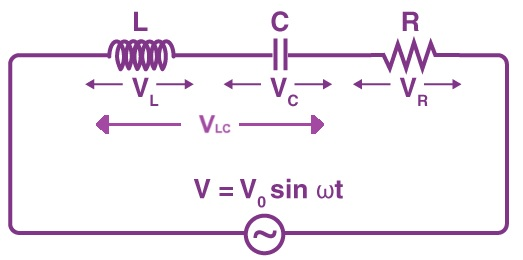
\includegraphics[width=0.7\columnwidth]{images/f1.jpg}
    \caption{Circuit diagram for the setup.}
    \label{fig:1}
\end{figure}

Here, $R_{dc}$ is the total d.c. resistance of the circuit that includes the resistance of the pure resistor, inductor and the internal resistance of the source, since the resistance of the inductor and source are not negligible as compared to the load resistance.

Also, $j\omega C$ and $1/j\omega C$ are the capacitive and inductive reactances of the capacitor and inductor respectively.

One can form a second order differential equation to describe the behaviour of a LCR circuit,

\begin{align}
    L\frac{d^2q}{dt^2}+R\frac{dq}{dt}+\frac{q}{C}=V_o\sin\omega t
\end{align}

By solving Eqn. (2) we can find the total impedance of the circuit,
\begin{align}
    I_o=\frac{V_o}{\vect{Z}}\implies\vect{Z} = \left[R_{dc} + j\left(\omega L-\frac{1}{\omega C}\right)\right]
\end{align}

Where its magnitude and phase are given by,
\begin{align}
    |\vect{Z}| &= \left[R^2_{dc} + \left(\omega L-\frac{1}{\omega C}\right)^2\right]^{1/2}\\
    \tan \phi &= \frac{\left(\omega L-\frac{1}{\omega C}\right)}{R_{dc}}
\end{align}

Where $\phi$ is the phase difference between the voltage across the source and the current in the circuit. From Eq. (5), we can arrive at 3 possible cases:

\paragraph*{\textbf{Case I:}} $\omega L > 1/\omega C$, tan $\phi$ is positive and applied voltage leads current by phase
angle $\phi$
\paragraph*{\textbf{Case II:}} $\omega L < 1/\omega C$, tan $\phi$ is negative and applied voltage lags current by phase
angle $\phi$
\paragraph*{\textbf{Case III:}} $\omega L = 1/\omega C$, tan $\phi$ is zero and applied voltage and current are in phase. Here, since $V_L = V_C$, the impedance, $Z$ is minimum, which means that the circuit is purely resistive. Also, current $I$ is maximum and $V_{LC}$ is minimum. This condition is known as \textbf{resonance}.\\

If $\omega_o$ is the frequency at which resonance occurs,
\begin{align}
    \omega_o L = 1/\omega_o C &\implies \omega_o = \frac{1}{\sqrt{LC}} \nonumber\\
    \text{or, } f_o &=  \frac{1}{2\pi\sqrt{LC}}
\end{align}

At resonant frequency, since the impedance is minimum, hence frequencies near $f_o$ are passed more readily than the other frequencies by the circuit. Due to this reason LCR series circuit is called \textbf{acceptor circuit}. The band of frequencies which is allowed to pass readily is called \textbf{pass-band}.

Conventionally, the band is chosen to be the range of frequencies between which the current is equal to or greater than $I_o/\sqrt{2}$. If $f_1$ and $f_2$ are the limiting
values of frequency as defined, then the width of the band (\textbf{bandwidth}) is $f_2 - f_1$.

The \textbf{selectivity} of a tuned circuit is its ability to select a signal at the resonant frequency and reject other signals that are close to this frequency. A measure of the selectivity is the quality factor (Q), which is defined as,
\begin{align}
    Q &= \frac{f_o}{f_2 - f_1} \\
    &= \frac{\omega_o L}{R_{dc}}=\frac{1}{R_{dc}\omega_o C}
\end{align}

In this experiment, we will probe the magnitude and phase of $V_R, V_{LC}, V_L, V_C$ in the vicinity of the resonant frequency of a LCR circuit. The working formulae for these quantities are,

\begin{align}
    \bigg|\frac{V_R}{V_i}\bigg| = \frac{R_{dc}}{|Z|} \text{ and, } &\phi_R = -\taninv{\left(\frac{\omega L-\frac{1}{\omega C}}{R_{dc}}\right)}\\
    \bigg|\frac{V_{LC}}{V_i}\bigg| &= \frac{\omega L-\frac{1}{\omega C}}{|Z|} \nonumber\\
    \text{ and, } \phi_{LC} &= \taninv{\left(\frac{R_{dc}}{\omega L-\frac{1}{\omega C}}\right)}\\
    \bigg|\frac{V_L}{V_i}\bigg| &= \frac{\omega L}{|Z|}\\
    \bigg|\frac{V_C}{V_i}\bigg| &= \frac{1/\omega C}{|Z|}
\end{align}

\subsection*{Applications}
Radio receivers, television sets, and oscillator circuits use LCR circuits for tuning purposes. These circuits mainly deal with the communication system and signal processing. The series LCR is used for voltage magnification. They are also used in induction heating.